\documentclass{article}
 
\usepackage{amsmath}
\usepackage{amssymb}
\usepackage{listings}
\usepackage{graphicx}
\usepackage{subcaption}
\usepackage{mwe}
\usepackage{float}
\usepackage{epstopdf}
\usepackage{outlines}
\usepackage[top=1.5in, bottom=1in, left=1in, right=1in]{geometry}


\title{Project 5 Extended Kalman Filters}

\begin{document}
\maketitle
\section{Project Goals}

The goals of this project are the following:\\\\
\begin{outline}[enumerate]
 \1 Estimate 2-D car position with sensor data and Kalman Filter.
 \1 Implement Kalman Filter on Lidar data and Extended Kalman Filter on Radar Data.
 \1 Compute Root Mean Squared Error to measure the difference between estimate and actual position.
\end{outline}

\section{Write up}
In this section I will briefly go over the C++ code and Environment setup. \\
\subsection{Kalman Filter with C++ } 
Three main files edited are \verb|kalman_filter.cpp|, \verb|FusionEKF.cpp| and \verb|tools.cpp|.\\

\begin{outline}[enumerate]
 \1 \verb|kalman_filter.cpp| follows the calculations in Figure \ref{fig1}, defines a Kalman Filter calculation object \verb|KalmanFilter| and several main function:
   \2 \verb|Init|: initializes Kalman Filter
   \2 \verb|Predict|: predicts the state and state covariance
   \2 \verb|Update|: update the state using standard Kalman Filter equations.
   \2 \verb|UpdateEKF|: update the state using Extended Kalman Filter equations.
   \2 \verb|UpdateCal|: includes the same equations used in both Kalman Filter and Exteneded Kalman Filter
\1 \verb|FusionEKF.cpp| reads the data from Lidar and Radar, calls Kalman Filter calculation object (\verb|ekf_| in the code) to get the Kalman Filter estimate Position. The overall processing flow is shown in Figure \ref{fig2}.
\1 \verb|tools.cpp| includes supporting function, Jacobian Matrix calculation and RMSE calculation.
\end{outline}

\begin{figure}[h!t]
\begin{center}
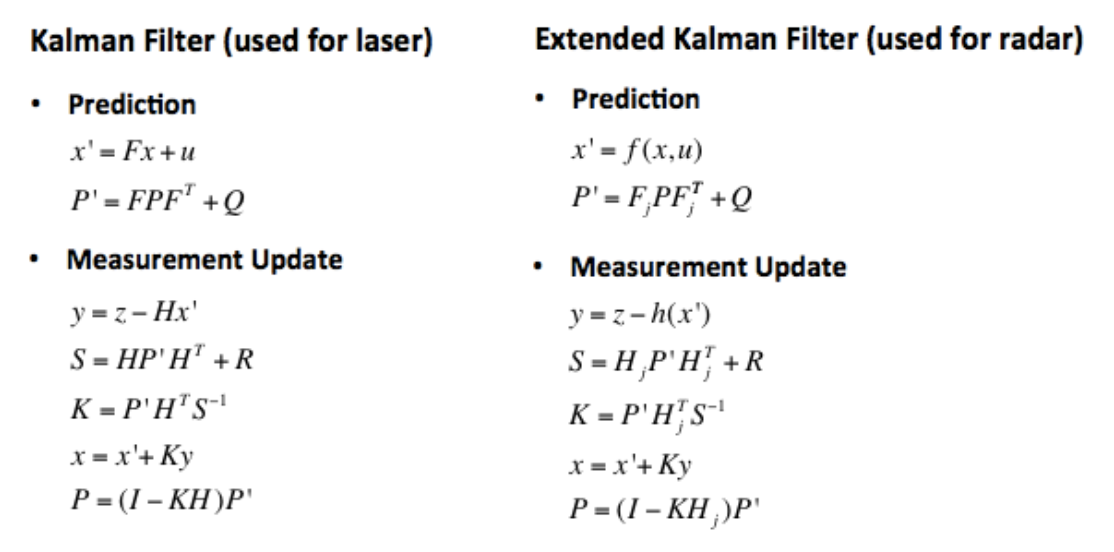
\includegraphics[width=0.75\textwidth]{Formula.png}
\caption{Kalman Filter Formulas}
\label{fig1}
\end{center}
\end{figure}

\begin{figure}[h!t]
\begin{center}
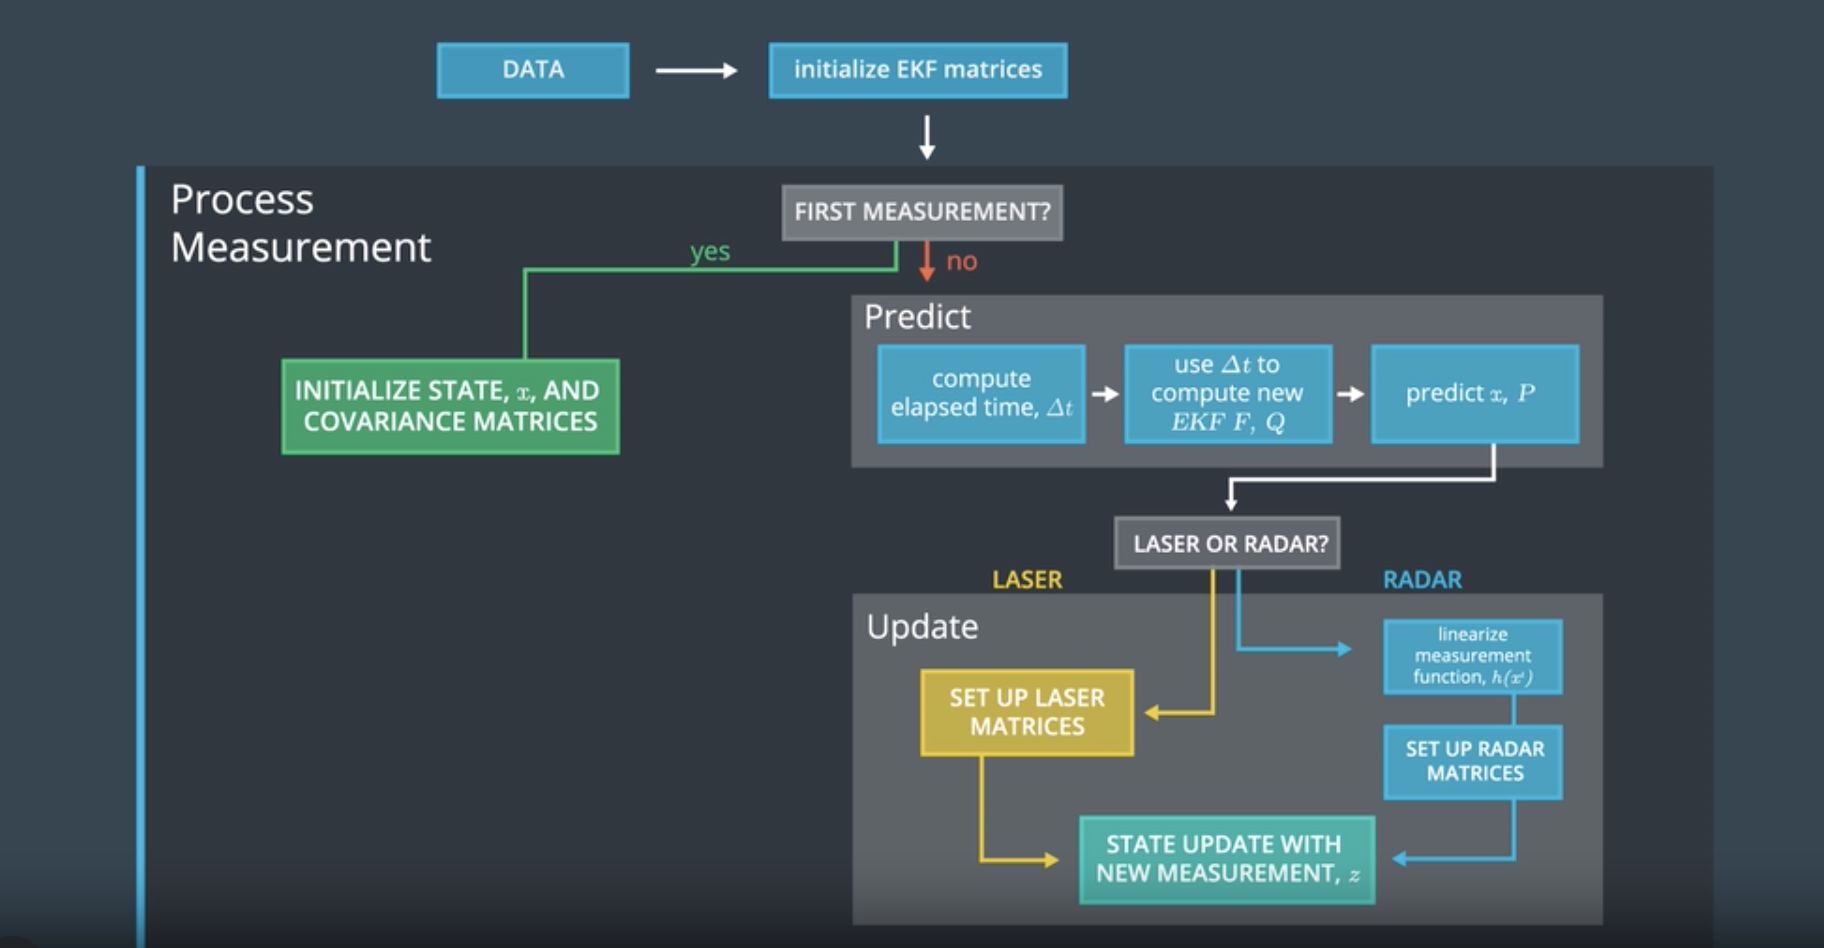
\includegraphics[width=0.75\textwidth]{Flow.png}
\caption{Sensor Fusion Process}
\label{fig2}
\end{center}
\end{figure}

\subsection{Environment setup} 

The setup in Mac is relative straightforward, download and extract term2 simulator and follow the instructions to compile the C++ code and connect the code to the simulator. 
\begin{itemize}
  \item{\verb|mkdir build|}
  \item{\verb|cd builf|}
  \item{\verb|cmake ..|}
  \item{\verb|make|}
  \item{\verb|./ExtendedKF|}
\end{itemize}

\subsection{Result} 
Final Result is shown in Figure \ref{fig3a} and Figure \ref{fig3b}. The px, py, vx, and vy RMSE for Dataset 1 and 2 is less than [.11, .11, 0.52, 0.52].

\begin{figure}
     \centering
     \begin{subfigure}[b]{0.4\textwidth}
         \centering
         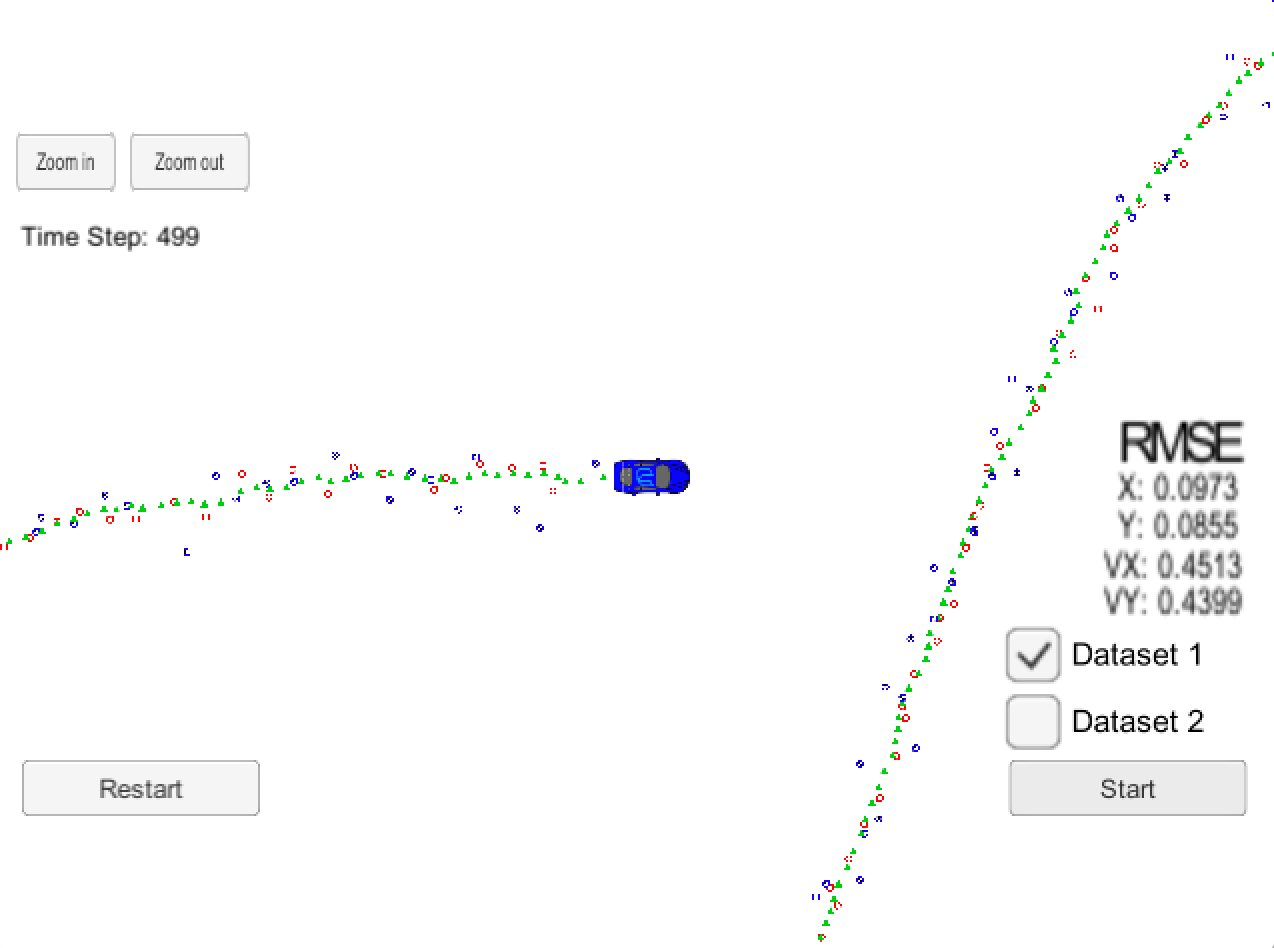
\includegraphics[width=\textwidth]{Test1.png}
         \caption{RMSE Dataset 1}
         \label{fig3a}
     \end{subfigure}
     \hfill
     \begin{subfigure}[b]{0.4\textwidth}
         \centering
         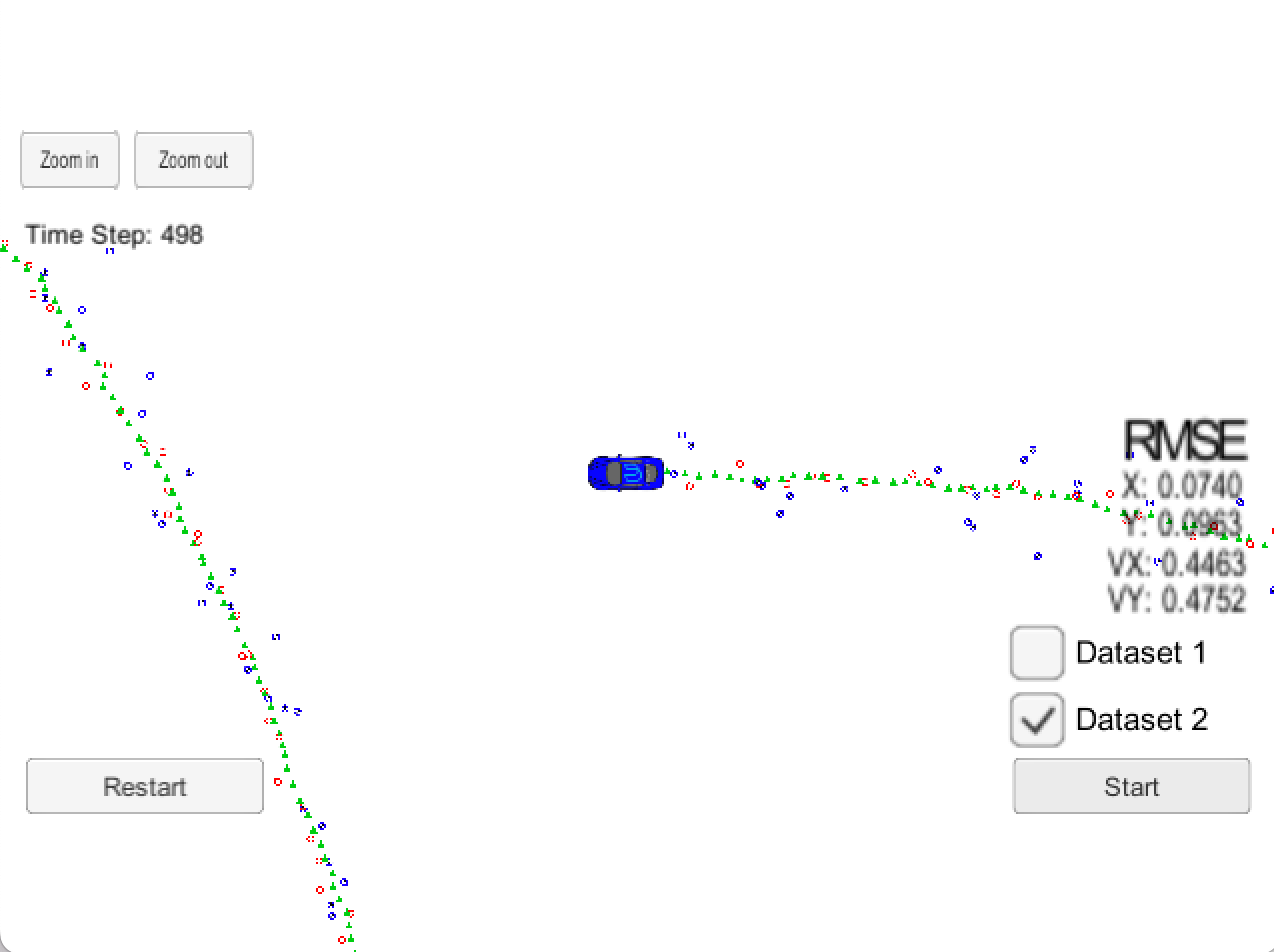
\includegraphics[width=\textwidth]{Test2.png}
         \caption{RMSE Dataset 2}
         \label{fig3b}
     \end{subfigure}
\end{figure}


\section{Discussion}
A bug I wrote is modifying P matrix calculation in the predict process again, P matrix is inherited from the last Kalman Filter iteration and there is no need to manually input it again.\\\\
A simple test is done by turning off Radar or Lidar calculation, from the RMSE result we can see estimate from Lidar is more accurate, and by fusing the data from Radar the accuracy is further improved.\\

\begin{figure}
     \centering
     \begin{subfigure}[b]{0.4\textwidth}
         \centering
         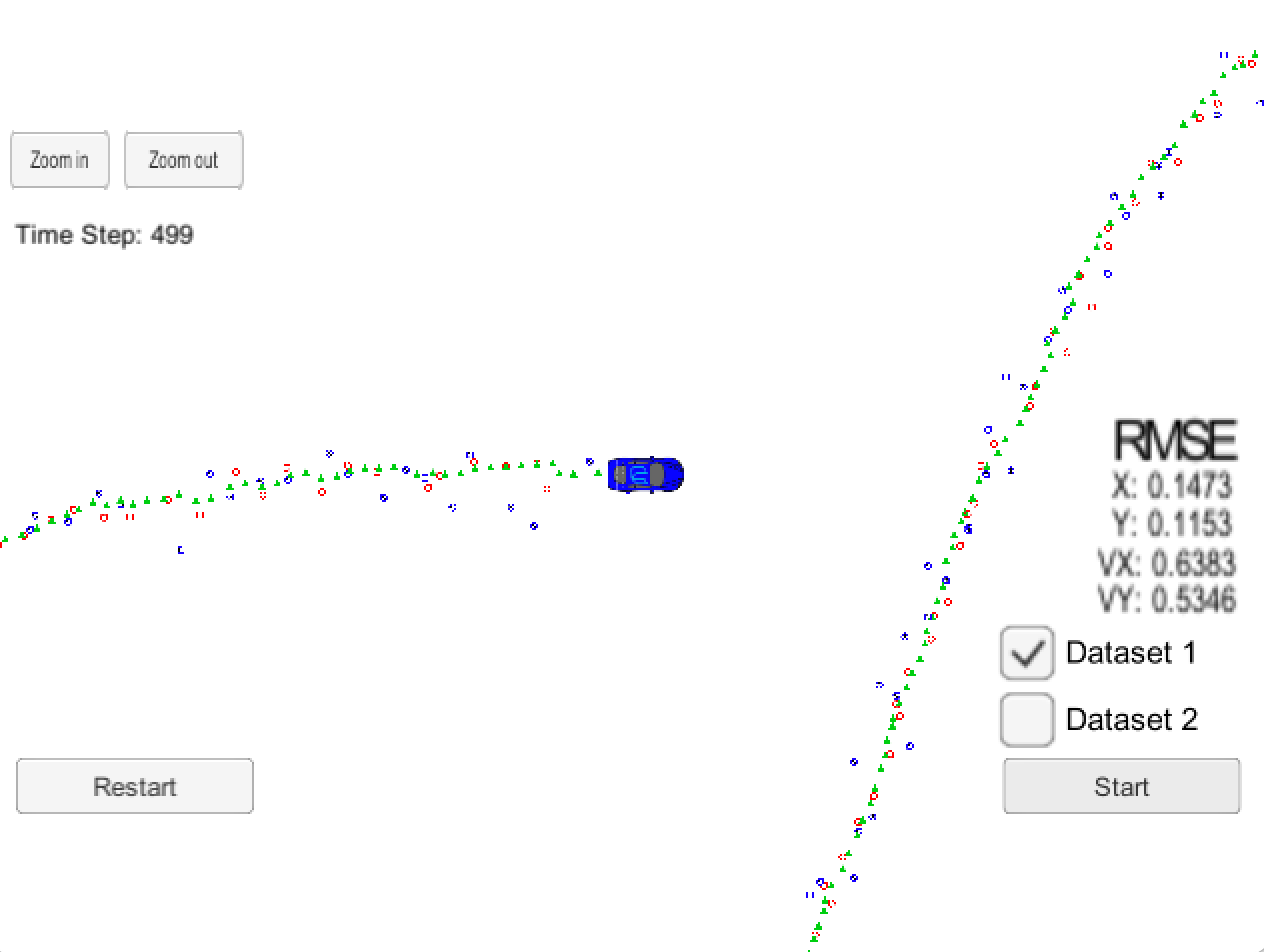
\includegraphics[width=\textwidth]{Lidar.png}
         \caption{Turn off Radar}
         \label{fig4a}
     \end{subfigure}
     \hfill
     \begin{subfigure}[b]{0.4\textwidth}
         \centering
         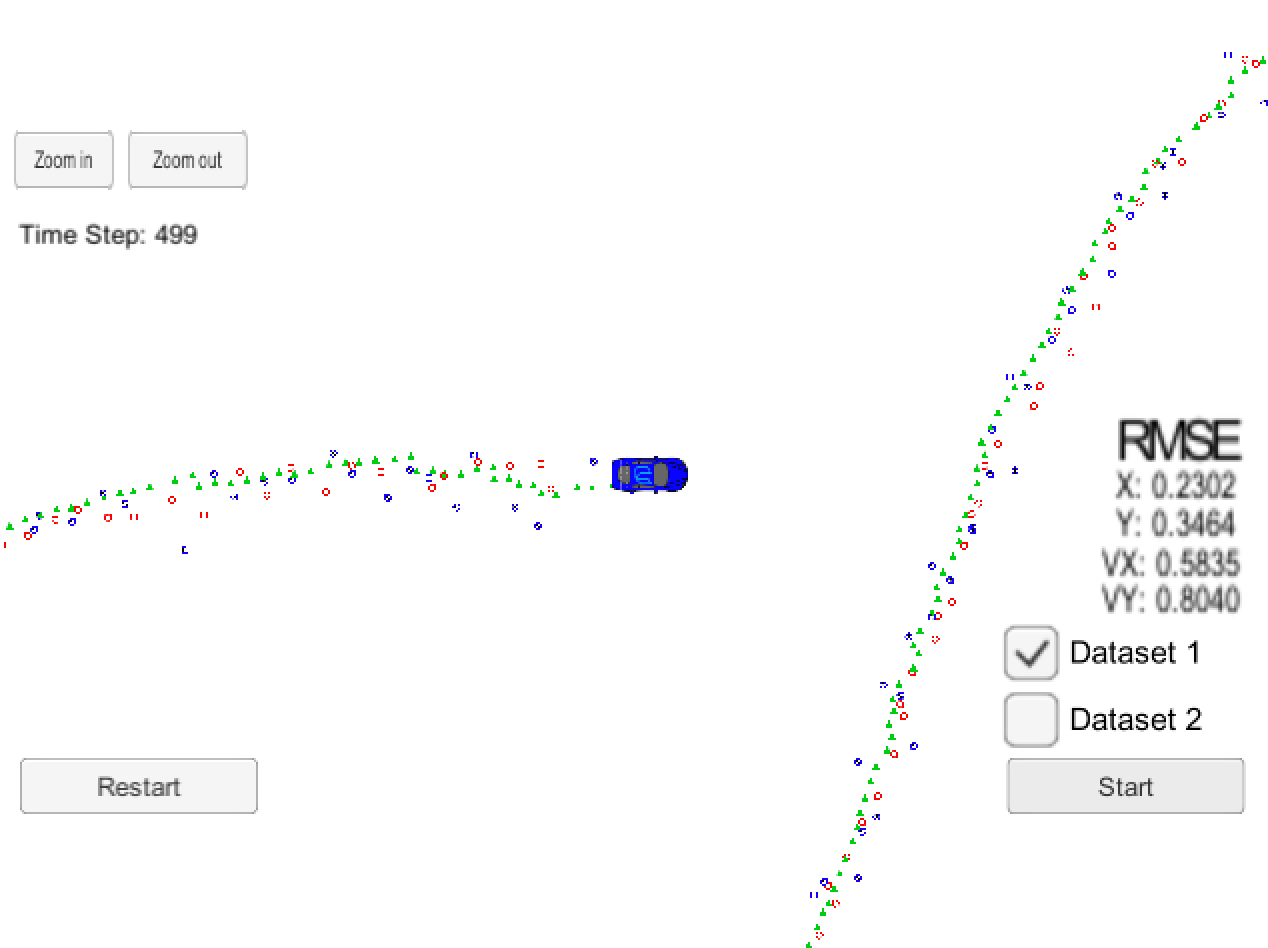
\includegraphics[width=\textwidth]{Radar.png}
         \caption{Turn off Lidar}
         \label{fig4b}
     \end{subfigure}
\end{figure}
\end{document}
